In this section, we evaluate RTSDP for two domains: \Invent~(Example 1) and \Mars~(Example 2). These domains show different challenges for planning as \Invent~contains continuously parametrised actions whereas \Mars~has a Nonlinear reward function.
We show the efficiency of our algorithm by comparing it with synchronous SDP.
The space efficiency is measured by the number of nodes in the XADD solution.
The time efficiency is measured by the convergency of the value of the initial state $s_0$.

\vspace{1mm}
\paragraph{\bf Example 2 (\Mars~NonLinear Domain) from \cite{sanner11} \label{ex2}}
\textit{This domain describes a planetary rover moving in a two dimensional plane (x, y), and searching for $k$ marked points from where it must take pictures.
There are also $k$ boolean $tp_i$ variables, one for each point, indicating whether the picture of point $i$ was already taken.
There is a single move action in this domain that simply reduces the distance from the rover to a specific point by $\frac{1}{3}$ of the current distance.
For all experiments, this target point was set to (0, 0).
The intent of this action is to represent the fact that a rover may move progressively more
slowly as it approaches a target position in order to reach the position with high accuracy.
There are $k$ $take-pic_i$ actions that provide reward according to nonlinear expressions over the continuous x and y variables, e.g. it is quadratically proportional to the distance from the picture point.
Hence for various points, the rover has to trade-off whether to take each picture at its current position or to get a larger reward by first moving and potentially getting closer before taking the picture. The reward for the $take-pic$ actions for a point in (0,0) is:
\begin{align*}
\small
R_{take-pic_i} (x, y, tp_i) =
\begin{cases}
  \text{if }  \neg tp_i \wedge x^2 + y^2 < 4 &: 4 - x^2 + y^2\\ 
  \text{otherwise} &:0,
\end{cases}
\end{align*} 
which shows that reward $r_i > 0$ is received at the first time the rover chooses take-pic and its distance to (0,0) is less than 2.
}

In Figure~\ref{fig:performance} the SDP plot shows the optimal initial state value for different stages-to-go, i.e. $V_h(s_0)$ is the value of the {\it h-th} point in the plot. 
The RTSDP plot is the estimated initial state value at the end of each trial, until the optimal value $V_H(s_0)$ is found.
Note that RTSDP reaches this optimal value much earlier than SDP and its value function has far fewer nodes.
Thus, our solver can achieve the optimal value for the initial state much faster and using a significantly smaller amount of memory space than synchronous SDP.

\vspace{-3mm}
\begin{figure}[ht]
\hspace{-2mm}
\subfloat[$V(s_0)$  $vs$ $Space$.]{
\includegraphics[width=1.65in]{figures/\perfOne/ValNodes.pdf}
}
\subfloat[$V(s_0)$ $vs$ $Time$.]{
\includegraphics[width=1.65in]{figures/\perfOne/ValTime.pdf}
}

\vspace{-4mm}
\hspace{-2mm}
\subfloat[$V(s_0)$  $vs$ $Space$.]{
\includegraphics[width=1.65in]{figures/\perfTwo/ValNodes.pdf}
}
\subfloat[$V(s_0)$ $vs$ $Time$.]{
\includegraphics[width=1.65in]{figures/\perfTwo/ValTime.pdf}
}

\vspace{-4mm}
\hspace{-2mm}
\subfloat[$V(s_0)$  $vs$ $Space$.]{
\includegraphics[width=1.65in]{figures/\perfThree/ValNodes.pdf}
}
\subfloat[$V(s_0)$ $vs$ $Time$.]{
\includegraphics[width=1.65in]{figures/\perfThree/ValTime.pdf}
}
\caption{CRTDP and SDP performance comparison on two domains \Invent ~($top$) and \Mars~($bottom$). Initial state value per memory ($left$) and time ($right$). SDP points are complete iterations (horizon) and RTSDP points are complete trials.}
\label{fig:performance}
\end{figure}

%\subsection{Solution behaviour}

Figures~\ref{invent2solution} and \ref{roverXY1solution} show the value functions for different stages-to-go generated by RTSDP and SDP when solving the \Invent~instance 2, with $H = 3$ and \Mars~instance 1, with $H=4$.
The SDP solutions {\it(right)} are the optimal value functions ($V_h^{DD(\vec{b},\vec{x})}$) shown as a 3D plot (continuous state variables X state value) and as an XADD. 
The RTSDP solutions {\it (left)} are the value functions obtained after a number of trials, such that the initial state value has converged to the optimal.
The RTSDP solver runs all trials from the initial state, so the value function for $H$ stages-to-go, $V_H$ {\it (bottom)} is always updated on the region containing the initial state.
As the updates refine the partition, the region containing $s_0$ shrinks.
Note that once a region no longer contains the initial state its heuristic value remains the same~(See Figures~\ref{invent2rtdp_plot3}, \ref{invent2rtdp_dd3}, \ref{roverXY1rtdp_plot4} and \ref{roverXY1rtdp_dd4}). In both domains, the use of reachability to prune updates is clear, there are plateaus on the unreachable regions that correspond to the initial heuristic, while the regions containing the initial state have a value similar to the optimal.

Another important comparison is how the solution size (number of XADD nodes) changes with the  number of stages-to-go. For the SDP~(Figures \ref{invent2sdp_dd1}, \ref{invent2sdp_dd2}, \ref{invent2sdp_dd3}, \ref{roverXY1sdp_dd1}, \ref{roverXY1sdp_dd3} and \ref{roverXY1sdp_dd4}), the complexity of the value function and solution size always increases quickly with horizon.
However, for RTSDP~(Figures \ref{invent2rtdp_dd1}, \ref{invent2rtdp_dd2}, \ref{invent2rtdp_dd3}, \ref{roverXY1rtdp_dd1}, \ref{roverXY1rtdp_dd3} and \ref{roverXY1rtdp_dd4}) there is different pattern: on one hand, as horizon increases the complexity of the solution in general does increase; On the other hand, if the number of performed actions is small, the number of reachable regions is also small and therefore the number of different terminal nodes and overall XADD size is not so large for the greater horizons. 

A peculiarity of this algorithm is that even though its solution is focused to obtain the initial state correct value, it provides useful information on many other states and stages-to-go, what makes it possible to be reused.

%\subfloat[RTSDP - $V^1$]{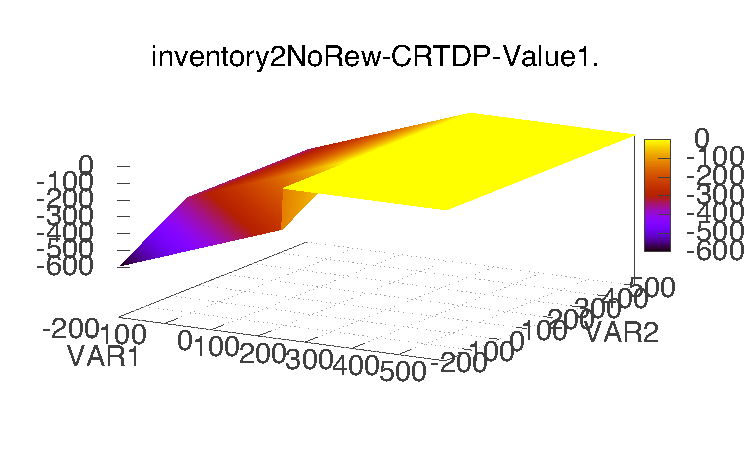
\includegraphics[width=0.28\linewidth, height=0.21\linewidth]{figures/\solutionExample/CRTDP-Value1.pdf}

\begin{figure*}[!ht]
\hspace{-5mm}
\subfloat[RTSDP - $V^1$]{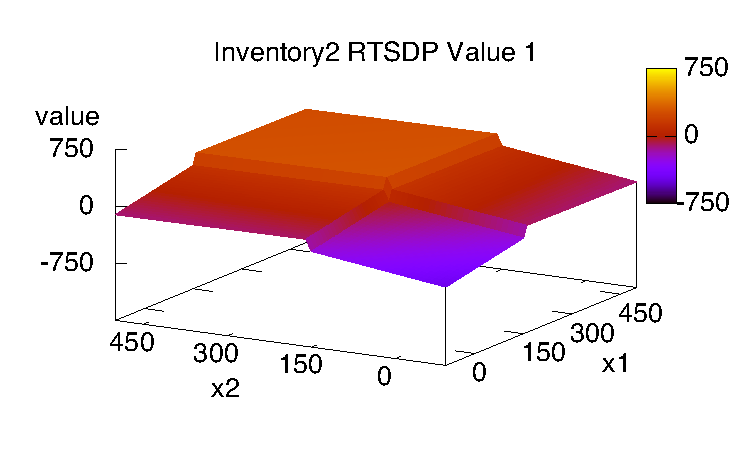
\includegraphics[width=0.28\linewidth, height=0.14\linewidth]{figures/\solutionExample/RTSDP-Value1.pdf}
\label{invent2rtdp_plot1}}
\subfloat[RTSDP - $DD^1$]{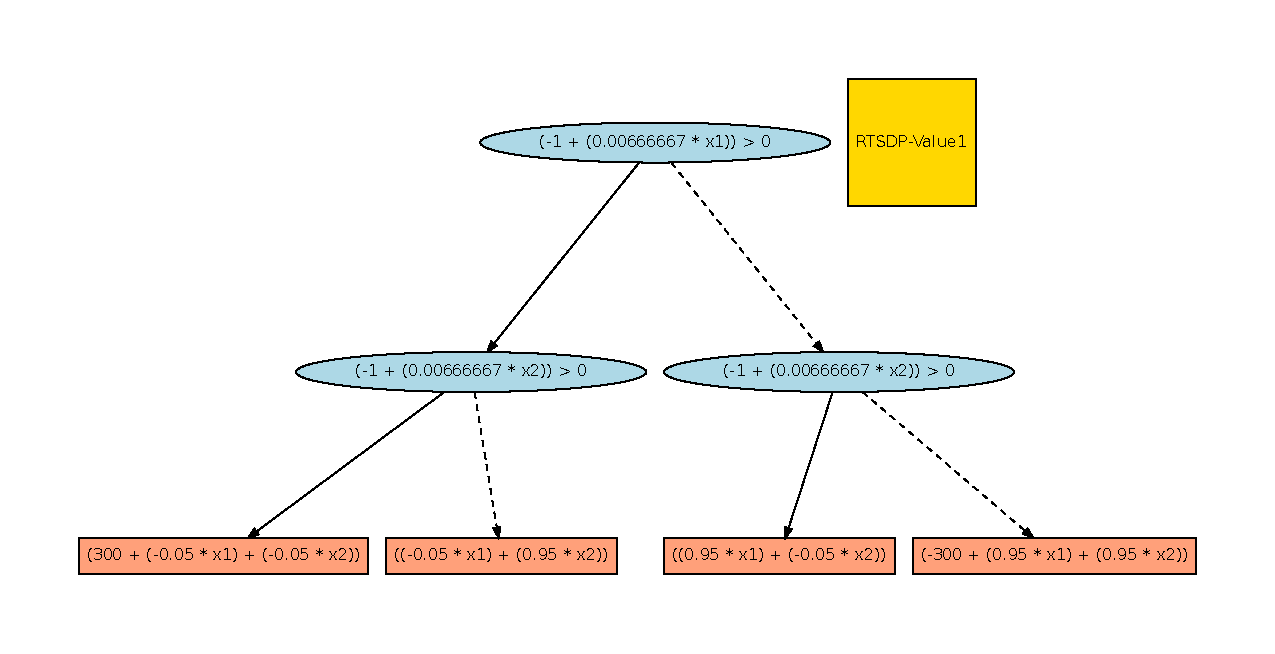
\includegraphics[width=0.24\linewidth, height=0.14\linewidth]{figures/\solutionExample/RTSDP-DD1.pdf}
\label{invent2rtdp_dd1}} 
\hspace{0.1cm}
\subfloat[SDP - $V^1$]{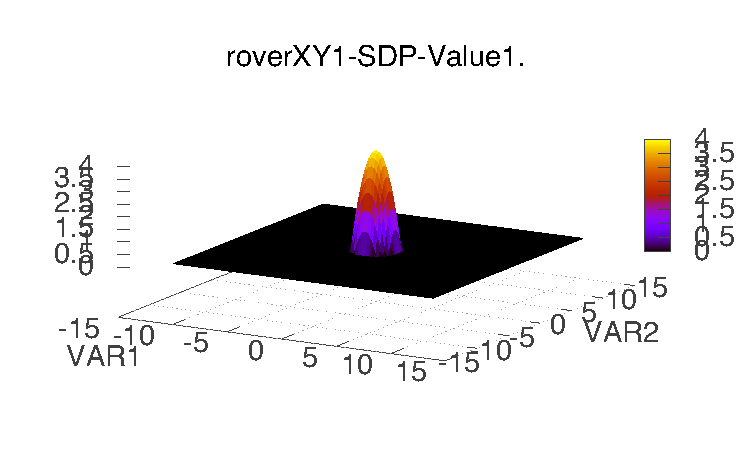
\includegraphics[width=0.28\linewidth, height=0.14\linewidth]{figures/\solutionExample/SDP-Value1.pdf}
\label{invent2sdp_plot1}}
\subfloat[SDP - $DD^1$]{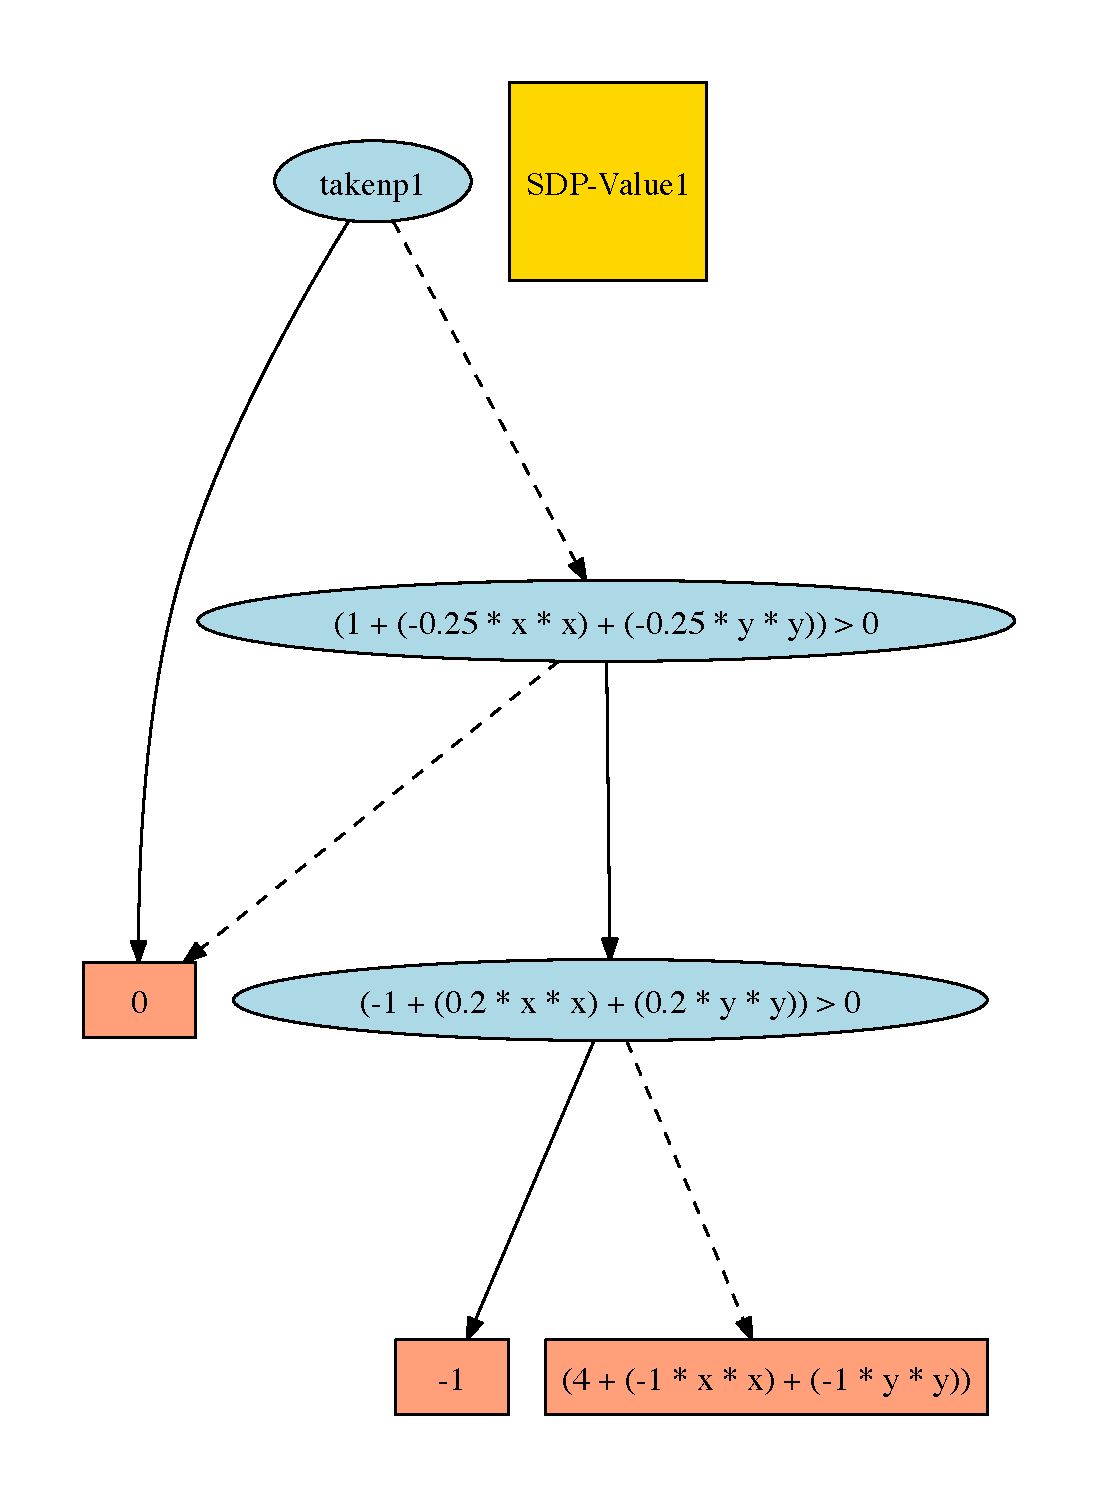
\includegraphics[width=0.24\linewidth, height=0.14\linewidth]{figures/\solutionExample/SDP-DD1.pdf}
\label{invent2sdp_dd1}} 

\hspace{-5mm}
\subfloat[RTSDP - $V^2$]{\includegraphics[width=0.28\linewidth, height=0.14\linewidth]{figures/\solutionExample/RTSDP-Value2.pdf}
\label{invent2rtdp_plot2}}
\subfloat[RTSDP - $DD^2$]{\includegraphics[width=0.24\linewidth, height=0.14\linewidth]{figures/\solutionExample/RTSDP-DD2.pdf}
\label{invent2rtdp_dd2}} 
\hspace{0.1cm}
\subfloat[SDP - $V^2$]{\includegraphics[width=0.28\linewidth, height=0.14\linewidth]{figures/\solutionExample/SDP-Value2.pdf}
\label{invent2sdp_plot2}}
\subfloat[SDP - $DD^2$]{\includegraphics[width=0.24\linewidth, height=0.14\linewidth]{figures/\solutionExample/SDP-DD2.pdf}
\label{invent2sdp_dd2}} 

\hspace{-5mm}
\subfloat[RTSDP - $V^3$]{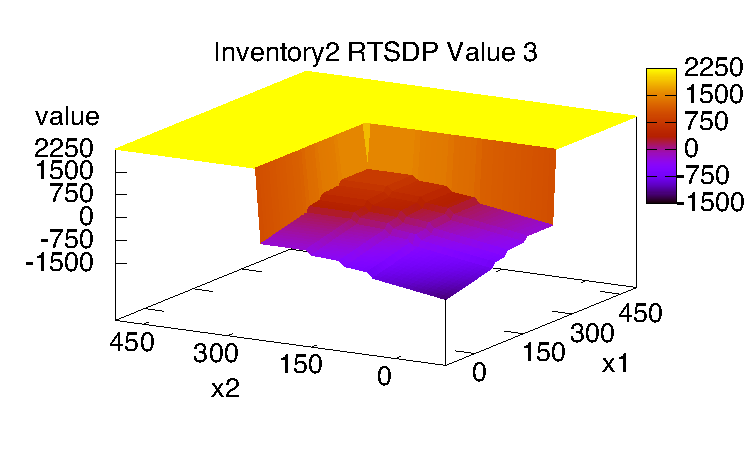
\includegraphics[width=0.28\linewidth, height=0.14\linewidth]{figures/\solutionExample/RTSDP-Value3.pdf}
\label{invent2rtdp_plot3}}
\subfloat[RTSDP - $DD^3$]{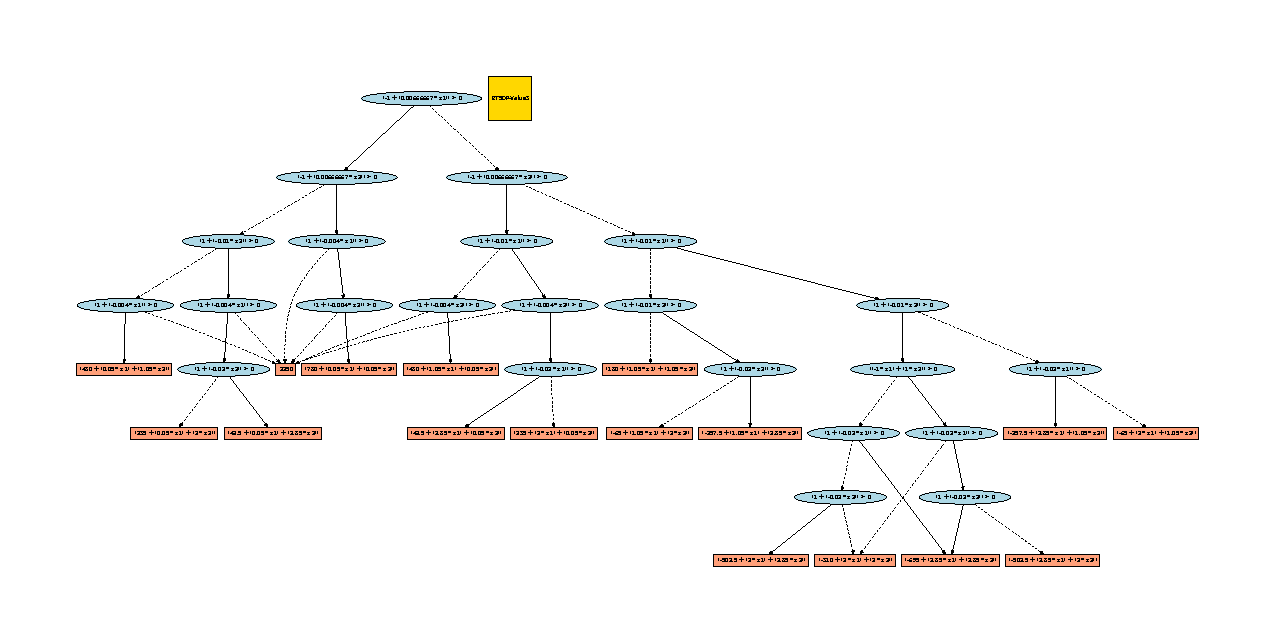
\includegraphics[width=0.24\linewidth, height=0.14\linewidth]{figures/\solutionExample/RTSDP-DD3.pdf}
\label{invent2rtdp_dd3}} 
\hspace{0.1cm}
\subfloat[SDP - $V^3$]{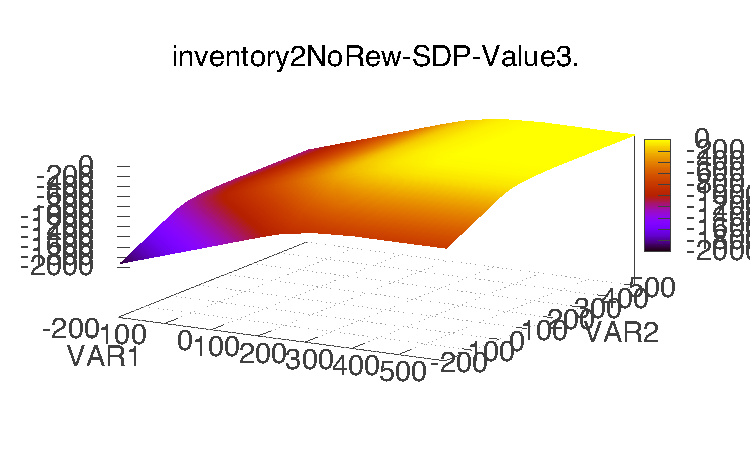
\includegraphics[width=0.28\linewidth, height=0.14\linewidth]{figures/\solutionExample/SDP-Value3.pdf}
\label{invent2sdp_plot3}}
\subfloat[SDP - $DD^3$]{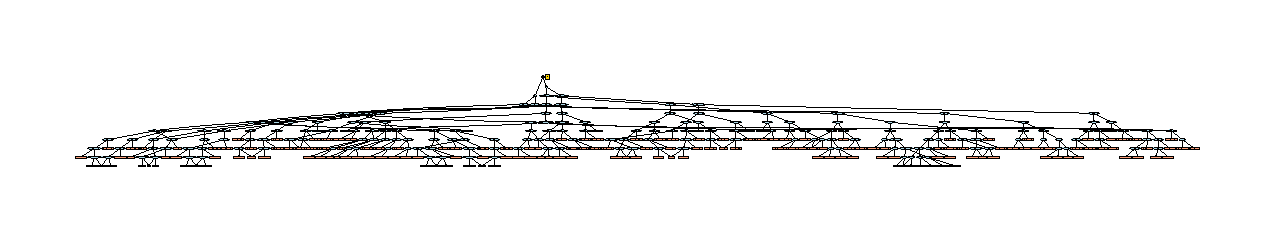
\includegraphics[width=0.24\linewidth, height=0.14\linewidth]{figures/\solutionExample/SDP-DD3.pdf}
\label{invent2sdp_dd3}} 

\hspace{-5mm}
\subfloat[RTSDP - $V^4$]{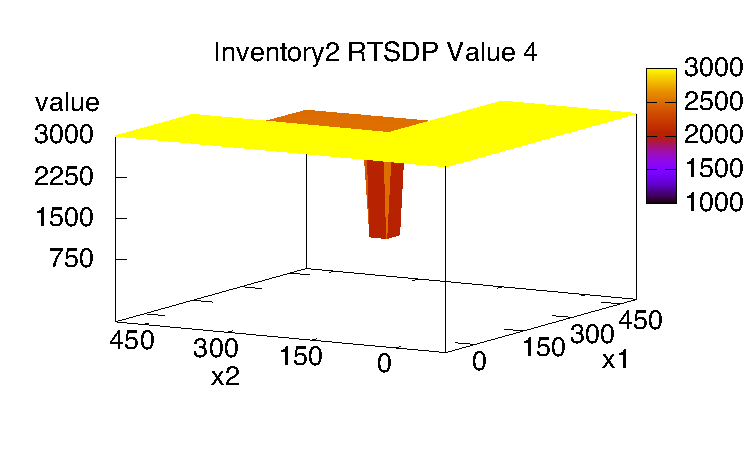
\includegraphics[width=0.28\linewidth, height=0.14\linewidth]{figures/\solutionExample/RTSDP-Value4.pdf}
\label{invent2rtdp_plot4}}
\subfloat[RTSDP - $DD^4$]{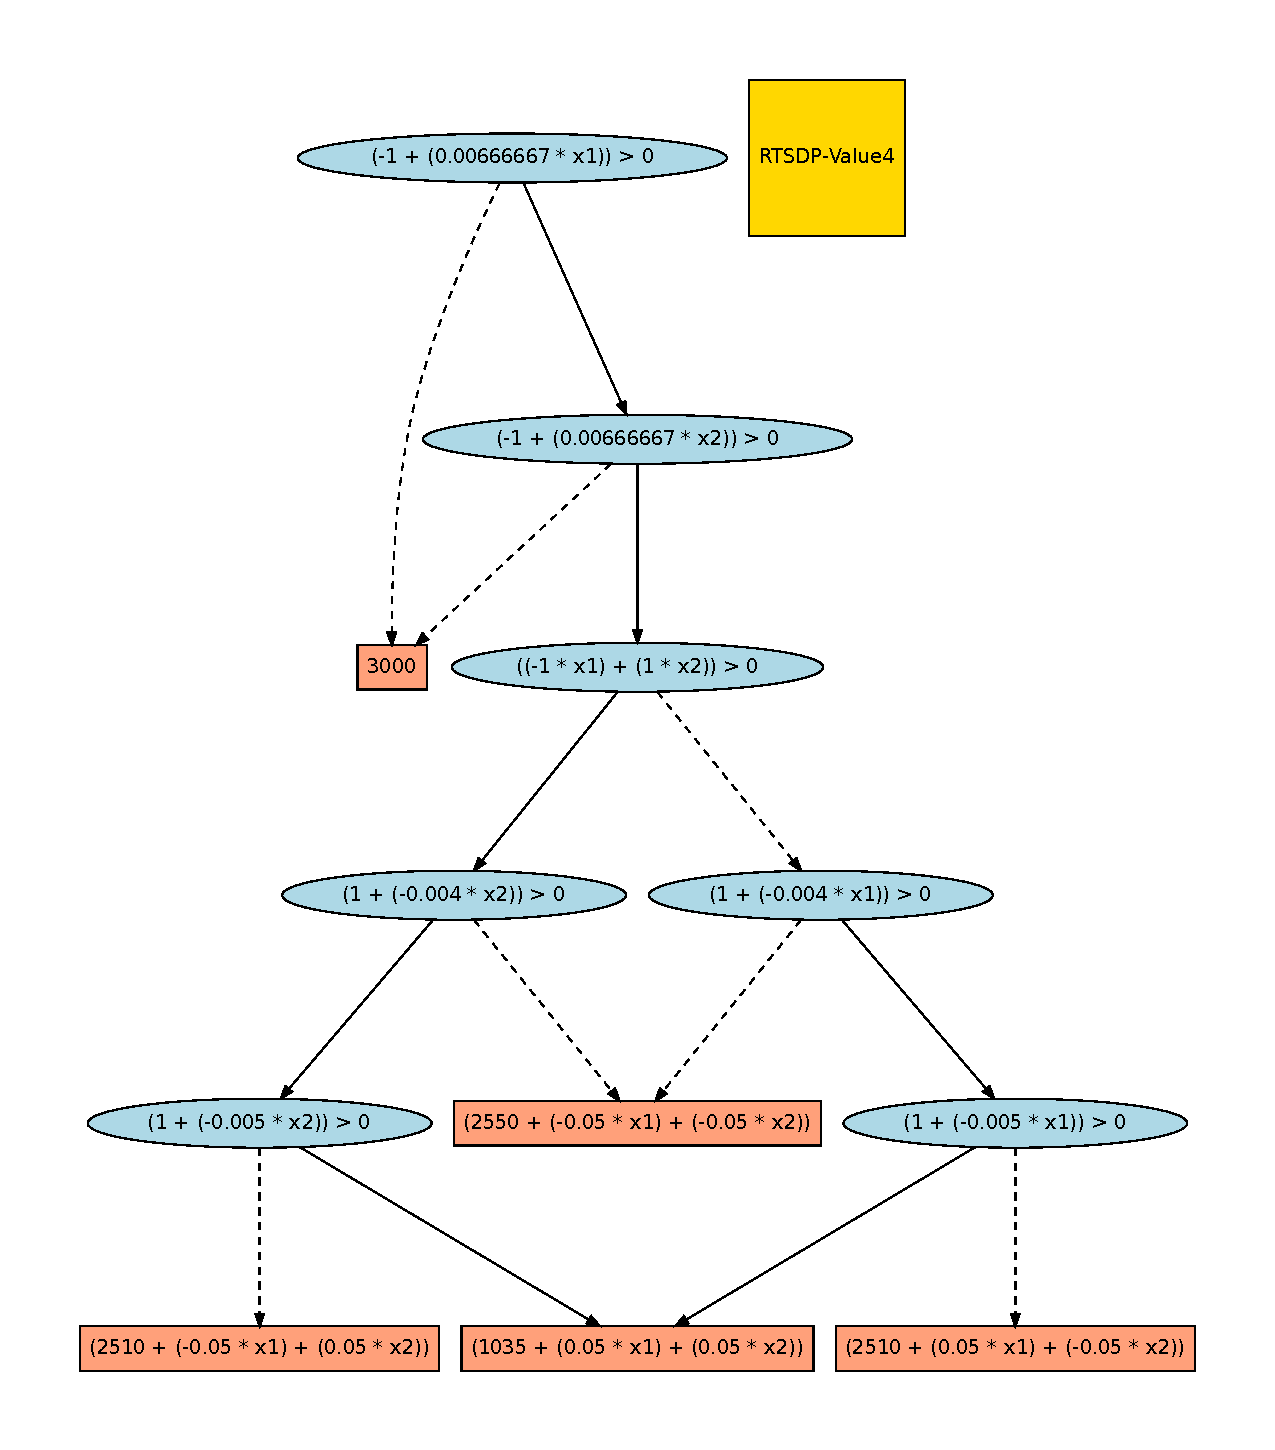
\includegraphics[width=0.24\linewidth, height=0.14\linewidth]{figures/\solutionExample/RTSDP-DD4.pdf}
\label{invent2rtdp_dd4}} 
\hspace{0.1cm}
\subfloat[SDP - $V^4$]{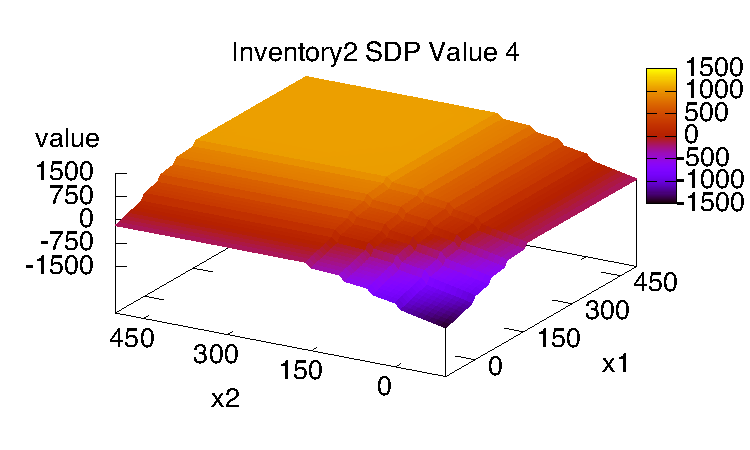
\includegraphics[width=0.28\linewidth, height=0.14\linewidth]{figures/\solutionExample/SDP-Value4.pdf}
\label{invent2sdp_plot4}}
\subfloat[SDP - $DD^4$]{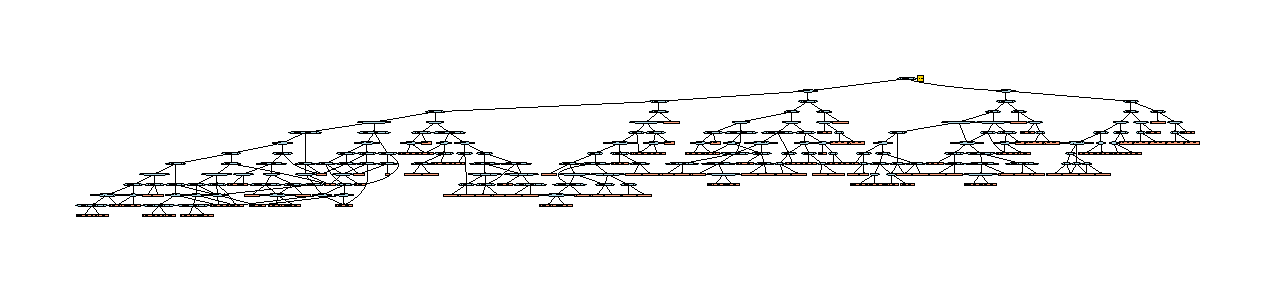
\includegraphics[width=0.24\linewidth, height=0.14\linewidth]{figures/\solutionExample/SDP-DD4.pdf}
\label{invent2sdp_dd4}} 
\caption{Value functions generated by RTSDP and SDP on \Invent, with $H=4$.}
\label{invent2solution}
\vspace{-6mm}
\end{figure*}

\begin{figure*}[!ht]
\hspace{-5mm}
\subfloat[RTSDP - $V^2$]{\includegraphics[width=0.28\linewidth, height=0.14\linewidth]{figures/\solutionExampleTwo/RTSDP-Value2.pdf}
\label{traffic1rtsdp_plot2}}
\subfloat[RTSDP - $DD^2$]{\includegraphics[width=0.24\linewidth, height=0.14\linewidth]{figures/\solutionExampleTwo/RTSDP-DD2.pdf}
\label{traffic1rtsdp_dd2}} 
\hspace{0.1cm}
\subfloat[SDP - $V^2$]{\includegraphics[width=0.28\linewidth, height=0.14\linewidth]{figures/\solutionExampleTwo/SDP-Value2.pdf}
\label{traffic1sdp_plot2}}
\subfloat[SDP - $DD^2$]{\includegraphics[width=0.24\linewidth, height=0.14\linewidth]{figures/\solutionExampleTwo/SDP-DD2.pdf}
\label{traffic1sdp_dd2}} 
\caption{Value 2 functions generated by RTSDP and SDP on \Traffic, with $H=2$.}
\vspace{-6mm}
\end{figure*}

\begin{figure*}[!ht]
\hspace{-5mm}
\subfloat[RTSDP - $V^2$]{\includegraphics[width=0.28\linewidth, height=0.14\linewidth]{figures/\solutionExampleThree/RTSDP-Value2.pdf}
\label{reservoir3rtsdp_plot2}}
\subfloat[RTSDP - $DD^2$]{\includegraphics[width=0.24\linewidth, height=0.14\linewidth]{figures/\solutionExampleThree/RTSDP-DD2.pdf}
\label{reservoir3rtsdp_dd2}} 
\hspace{0.1cm}
\subfloat[SDP - $V^2$]{\includegraphics[width=0.28\linewidth, height=0.14\linewidth]{figures/\solutionExampleThree/SDP-Value2.pdf}
\label{reservoir3sdp_plot2}}
\subfloat[SDP - $DD^2$]{\includegraphics[width=0.24\linewidth, height=0.14\linewidth]{figures/\solutionExampleThree/SDP-DD2.pdf}
\label{reservoir3sdp_dd2}} 
\caption{Value 2 functions generated by RTSDP and SDP on \Reservoir, with $H=2$.}
\vspace{-6mm}
\end{figure*}

\input tablesp